\subsection{Erkenntnisse}

\begin{frame}
  \begin{itemize}
    \item erstmal auf allgemeine Erkenntnisse eingehen
  \end{itemize}
\end{frame}

\begin{frame}
  \frametitle{\currentsectionname}

  \begin{figure}
    \pgfplotstableread[col sep=comma]{assets/study-results.csv}\datatable
\centering
\resizebox{.95\textheight}{!}{%
  \begin{tikzpicture}
    \begin{axis}[
        boxplot/draw direction=y,
        boxplot/every median/.style={ultra thick},
        xtick={1,2,3},
        xticklabels={Szenario 1, Szenario 2, Szenario 3},
        ytick={1,...,7},
        ymin=1,
        ylabel={SEQ},
      ]
      \addplot+ [boxplot, plot1] table [y=a] {\datatable};
      \addplot+ [boxplot, plot2] table [y=b] {\datatable};
      \addplot+ [boxplot, plot3] table [y=c] {\datatable};
    \end{axis}
  \end{tikzpicture}
}

    \caption{Antworten auf die Single Ease Question nach jedem Szenario (1: sehr schwer, 7: sehr einfach).}
  \end{figure}

  % \note{
  %   \begin{itemize}
  %   \end{itemize}
  % }

\end{frame}

\begin{frame}

  \begin{figure}
    \pgfplotstableread[col sep=comma]{assets/study-results.csv}\datatable
\centering
\resizebox{.95\textheight}{!}{%
  \begin{tikzpicture}
    \begin{axis}[
        boxplot/draw direction=y,
        boxplot/every median/.style={ultra thick},
        xtick={1,2},
        xticklabels={Vorversion, Block-Editor},
        ytick={1,...,10},
        ymin=1,
        ylabel={Einfachheit der Benutzung},
      ]
      \addplot+ [boxplot, plot1] table [y=prev] {\datatable};
      \addplot+ [boxplot, plot2] table [y=ges] {\datatable};
    \end{axis}
  \end{tikzpicture}
}

    \caption{Einschätzung der Einfachheit der Benutzung nach dem Usability Test auf einer Skala von 1 (sehr schwer) bis 10 (sehr einfach).}
  \end{figure}

\end{frame}

\begin{frame}

  \begin{figure}
    \colorlet{presentation}{plot1}
\colorlet{interaction}{plot2}
\colorlet{content}{plot3}
\colorlet{technical}{plot4}
\centering
\resizebox{.75\textheight}{!}{%
  \begin{tikzpicture}
    \begin{axis}[
        xbar=0pt,
        xmajorgrids=true,
        xtick={0,...,10},
        xmin=0,
        xmax=6,
        xlabel={Absolute Häufigkeit},
        /pgf/bar shift=0pt,
        legend style={legend cell align=left},
        legend pos=south east,
        axis y line*=none,
        axis x line*=bottom,
        tick label style={font=\footnotesize},
        legend style={font=\footnotesize},
        label style={font=\footnotesize},
        width=.6\textwidth,
        bar width=3.5mm,
        ymin=1,
        ytick={1,...,20},
        ytick style={draw=none},
        yticklabels={
            {Übersichtlichkeit Funktionsliste},
            {Präfix von Objektklassen},
            {Details zu Funktionen},
            {Benennung Abfragbare Felder},
            {Probleme mit Scrollen},
            {Zugriff auf die Quelldaten},
            {Automatische Typ-Filterung},
            {Angabe von statischen Werten},
            {Auswahl von Überladungen},
            {Benennung rechter Bereich},
            {Benennung des Speichern-Buttons},
            {Parameterübernahme bei Überladungen},
            {Drag and Drop},
            {Ersetzen von Einträgen},
            {Details zu Parametern},
            {Metadaten von Szenario-Feldern},
            {Anzeige von Attributen in Ziel},
            {Datentyp von Szenario-Feldern},
            {Symbole für Datentypen},
            {Bedienreihenfolge von Funktionen},
          },
        area legend,
        y=6mm,
        enlarge y limits={abs=0.625},
        every axis plot/.append style={fill}
      ]
      \addplot[interaction]  coordinates {(0,0)};  \addlegendentry{Interaktion (8)}
      \addplot[presentation] coordinates {(0,0)};  \addlegendentry{Darstellung (7)}
      \addplot[content]      coordinates {(0,0)};  \addlegendentry{Inhalt (4)}
      \addplot[technical]    coordinates {(0,0)};  \addlegendentry{Technisch (1)}

      \addplot[presentation] coordinates {(1,1)};  % Übersichtlichkeit Funktionsliste
      \addplot[content]      coordinates {(2,2)};  % Präfix von Objektklassen
      \addplot[content]      coordinates {(2,3)};  % Details zu Funktionen
      \addplot[presentation] coordinates {(2,4)};  % Benennung Abfragbare Felder
      \addplot[technical]    coordinates {(3,5)};  % Probleme mit Scrollen
      \addplot[content]      coordinates {(3,6)};  % Zugriff auf die Quelldaten
      \addplot[interaction]  coordinates {(3,7)};  % automatische Typ-Filterung
      \addplot[interaction]  coordinates {(3,8)};  % Angabe von statischen Werten
      \addplot[interaction]  coordinates {(3,9)};  % Auswahl von Überladungen
      \addplot[presentation] coordinates {(4,10)}; % Benennung rechter Bereich
      \addplot[presentation] coordinates {(4,11)}; % Benennung des Speichern-Buttons
      \addplot[interaction]  coordinates {(4,12)}; % Parameterübernahme bei Überladungen
      \addplot[interaction]  coordinates {(4,13)}; % Drag and Drop
      \addplot[interaction]  coordinates {(4,14)}; % Ersetzen von Einträgen
      \addplot[content]      coordinates {(5,15)}; % Details zu Parametern
      \addplot[presentation] coordinates {(5,16)}; % Metadaten von Szenario-Feldern
      \addplot[presentation] coordinates {(5,17)}; % Anzeige von Attributen in Ziel
      \addplot[interaction]  coordinates {(5,18)}; % Datentyp von Szenario-Feldern
      \addplot[presentation] coordinates {(6,19)}; % Symbole für Datentypen
      \addplot[interaction]  coordinates {(6,20)}; % Bedienreihenfolge von Funktionen
    \end{axis}
  \end{tikzpicture}
}

    \caption{Häufigkeit des Auftretens verschiedener Usability-Probleme.}
  \end{figure}

\end{frame}

\begin{frame}

  BEDIENREIHENFOLGE FUNKTIONEN VERGLEICHEN

\end{frame}

\begin{frame}

  \begin{figure}
    \centering
\begin{tikzpicture}
  \tikzset{icon/.style={outer xsep=4.5em, outer ysep=1em, minimum height=3em}}
  \tikzset{label/.style={font=\footnotesize}}
  \node [icon] (text)  at (0, 0)       {\includesvg[width=2em]{assets/bi-card-text.svg}};
  \node [icon] (int)   at (text.east)  {\includesvg[width=2em]{assets/bi-123.svg}};
  \node [icon] (float) at (int.east)   {\includesvg[width=2em]{assets/bi-123.svg}};
  \node [icon] (bool)  at (float.east) {\includesvg[width=2em]{assets/bi-toggles.svg}};
  \node [icon] (dt)    at (bool.east)  {\includesvg[width=2em]{assets/bi-calendar-week.svg}};
  \node [icon] (geom)  at (dt.east)    {\includesvg[width=2em]{assets/bi-pin-map.svg}};
  \node [label] at (text.south)  {Text};
  \node [label] at (int.south)   {Ganzzahl};
  \node [label] at (float.south) {Gleitkommazahl};
  \node [label] at (bool.south)  {Boolean};
  \node [label] at (dt.south)    {Datum/Zeit};
  \node [label] at (geom.south)  {Geometrie};
\end{tikzpicture}

    \caption{Die im Block-Editor verwendeten Symbole für Datentypen.}
  \end{figure}

  \begin{itemize}
    \item Verwechselung von Ganzzahl und Gleitkommazahl
    \item Symbol für Boolean wurde als Schaltflächen identifiziert
  \end{itemize}

  \Note{
    \item Verwechselung auch von Menschen mit Programmierkenntnisse
    \item Boolean-Problem Oft schon beim ersten Eindruck genannt
  }

\end{frame}

\begin{frame}

  \begin{figure}
    \begin{center}
      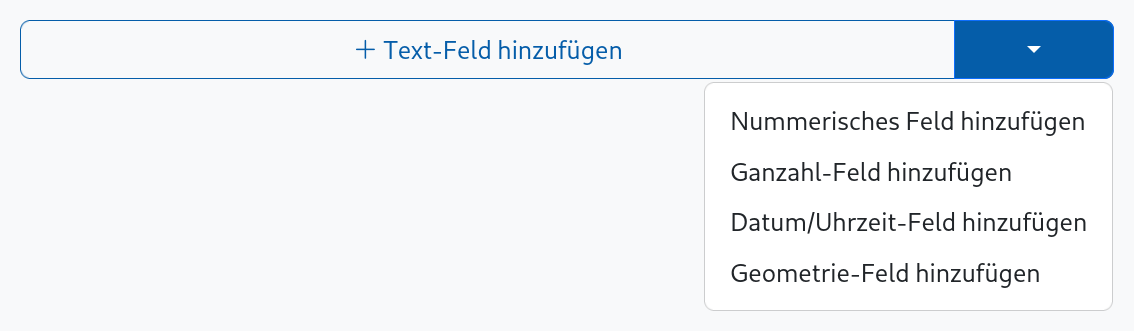
\includegraphics[width=0.95\textwidth]{assets/datatype-dropdown.png}
    \end{center}
    \caption{Dropdown-Menü zum Auswählen des Datentyps von Feldern.}
  \end{figure}

\end{frame}

\begin{frame}

  ZUSAMMENFASSEN VON ANDEREN PROBLEMEN, "GRÖßTE" RAUSSUCHEN

\end{frame}
